
\begin{frame}
  \frametitle{Motivation}
  \framesubtitle{ZENO/Walk-on-Spheres}

  \begin{figure}
    \centering
    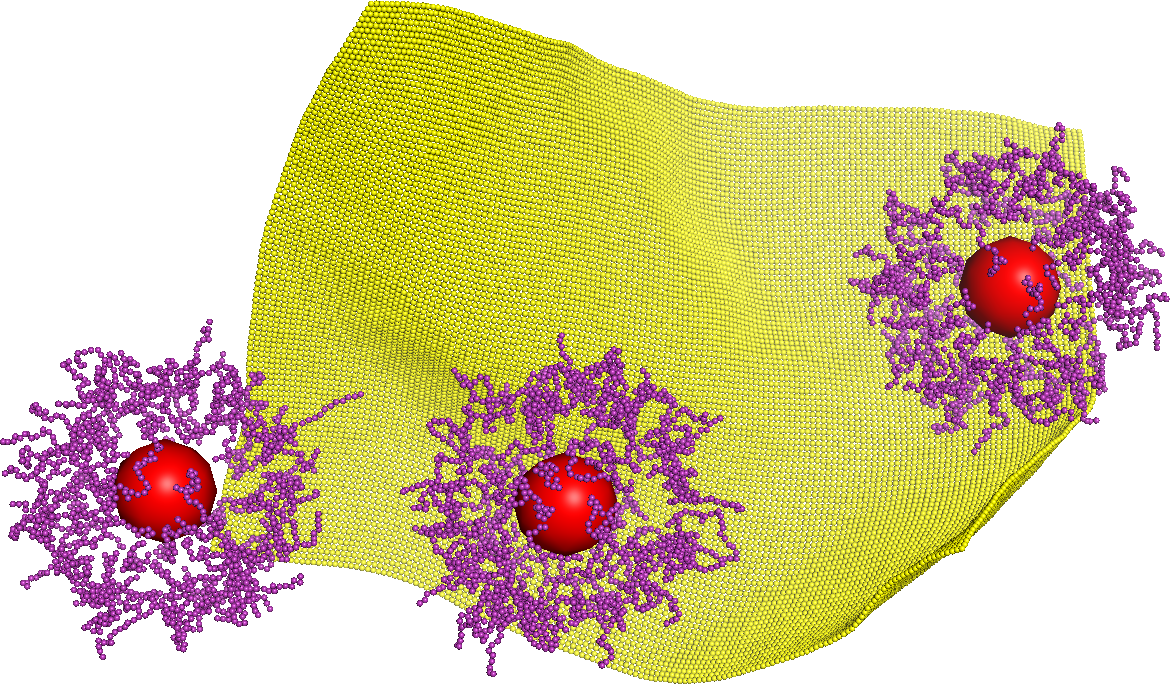
\includegraphics[width=0.7\textwidth]{80000_NOBGCROP.png}
    \caption{DNA-grafted gold nano-particles interacting with a 
    two-dimensional DNA-based origami construct (23115 speheres).}
    \label{fig:80000}
  \end{figure}
\end{frame}

\begin{frame}
  \frametitle{Motivation}
  \framesubtitle{ZENO/Walk-on-Spheres}

  \begin{itemize}
    \item Walk-on-Spheres accelerates Brownian Motion by jumping to a uniformly distributed point on the surface
      of a surrounding sphere
      \begin{itemize}
        \item The radius of the surrounding sphere is the distance of the random walker to the molecule
        \item Our implementation uses \kd trees to quickly find the nearest neighbor
      \end{itemize}
    \item The random access pattern of a \kd tree limits its potential for use on GPUs where memory operations
      are highly costly
  \end{itemize}

\end{frame}

\begin{frame}
  \frametitle{Specification}

  {\usebeamerfont{title}\color{white}
  Improve performance of nearest neighbor search on \kd trees by more compactly organizing tree components
  to reduce cache misses and load instructions.}

\end{frame}
